\section{Formalisation}
\label{sec:Formalisation}

Our formal framework defines a \emph{paradigm} as a \emph{label}/\emph{name} 
$\iota$ denoting a set of properties $\pi\in\Pi$. We define a 
\emph{paradigmatic structure} $\mathsf{PS}\in \PS$ as a candidate structure that 
\emph{qualifies}, or \emph{embodies}, or \emph{follows} the paradigm $\iota$ if 
$\mathsf{PS}$ satisfies $\pi$. $\mathsf{PS}$ describes a set of workflows that 
describe various activities that are seen to be desirable for realising 
$\iota$. 

Since every aspects of the paradigmatic structure need to be explicitly 
modelled, we first introduce the two classical notions to manipulate languages 
explicitly, namely metamodels and models on the one hand, and transformation 
specification and execution on the other. 

A \emph{metamodel} $\mathsf{MM} \in \mathcal{M}$ specifies the \emph{abstract 
syntax} of a language $\mathsf{L}$. $\mathsf{MM}$ is expressed in a specific 
language called meta-metamodel. 
A \emph{model} $\mathsf{M} \in \mathbb{M}$ is a particular instance of 
$\mathsf{L}$, also specified using a language that may be visual / 
diagrammatic, textual or hybrid (and normally different from the 
meta-metamodel). When $\mathsf{M}$ is a valid instance of 
$\mathsf{MM}$, $\mathsf{M}$ is said to \emph{conform to} $\mathsf{MM}$ and noted 
$\mathsf{M} \rhd \mathsf{MM}$. 

A \emph{transformation specification} $\mathsf{T}\in\mathbb{T}$ is a triple 
$\mathsf{T} = ((\mathsf{MM_s^{i}})_{\mathsf{i}\in [1..n]}, 
(\mathsf{MM_t^{j}})_{\mathsf{j}\in[1..m]}, \mathsf{spec})$, where  
$(\mathsf{MM_s^{i}})_{\mathsf{i}\in [1..n]}$ and
$(\mathsf{MM_t^{j}})_{\mathsf{j}\in [1..m]}$ are indexed sets of source and
target languages, respectively, and constitute the transformation's 
\emph{signature}; while $\mathsf{spec}$ is a well-formed 
transformation definition written in a transformation language. A 
\emph{transformation execution} $\mathsf{TE_{T}}\in\TE$ is a general 
computation performed on (a) language instance(s) that conform(s) to the 
source language(s) of the transformation $\mathsf{T}\in\mathbb{T}$.

As an example, the $\mathsf{javac}$ compiler is a transformation 
$\mathsf{T}_{compil} = (\mathsf{MM_{Java}}, \mathsf{MM_{BC}}, \mathsf{javac})$
that outputs byte code (BC) from any (valid, conforming) Java program 
$\mathsf{J}  \rhd \mathsf{MM_{Java}}$. Note that $\mathsf{javac}$ is itself 
specified as a Java program (i.e. $\mathsf{javac} \rhd \mathsf{MM_{Java}}$).

\subsection{Templates}
\label{sec:Templates}

Templates are plain metamodels and transformations, specified with the usual 
meta-metamodel(s) and transformation languages. A key difference however is 
that they are not complete, in the sense that they require a regular metamodel 
(or transformations) to be matched. Templates are used as placeholders for 
enforcing transformation signatures, expressing high-level properties for 
metamodels and transformations (specifications), or capturing the necessary 
steps in a transformation. 
\begin{wrapfigure}[14]{r}{0.1\textwidth}
  \begin{center}
    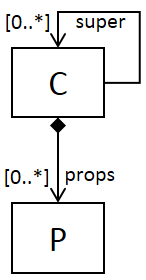
\includegraphics[width=0.1\textwidth]{InheritenceTemplate}
  \end{center}
  \caption{Simple Class-Property Template for capturing Inheritance.}
  \label{fig:InheritenceTemplate}
\end{wrapfigure}
Suppose we want to formally specify Property $\mbox{OO}_3$ for inheritance in 
Table \ref{tab:Properties}. Figure \ref{fig:InheritenceTemplate} presents a 
minimal template defining the basic placeholders: to even allow discussing 
about super- and sub-classes, one need at least distinguishing between 
$\mathsf{C}$lass and Objects, and defining a partial order ($\mathsf{super}$) 
between classes. The inheritance property then states that any object of a 
subclass has access to the state defined by its class, but also to the state 
defined by its superclass. Note that using a \textsc{Mof}-like meta-metamodel 
for expressing the template provides navigational notation for free: the 
property would start with something like $\mathsf{c1, c2 : Class}$ such that 
$\mathsf{c2} \in \mathsf{c1.super}$.

Using templates requires a powerful, customisable matching process. For 
metamodels, contributions on model typing \cite{J:Degueule-etAl:2017}, a 
posteriori typing \cite{J:deLara-Guerra:2017}, and metamodel morphisms 
\cite{Salay-Mylopoulos-Esterbrook:2008,Duran-Zschaler-Troya:2012} may be 
appropriate; for transformations, the rich literature on reuse 
\cite{J:Kusel-etAl:2015} provides some guidelines on how to realise that. Hence, 
matching Fig. \ref{fig:InheritenceTemplate}'s template into the Java 
metamodel \cite{B:Java:2019} would match $\mathsf{ClassDeclaration}$ to 
$\mathsf{C}$ and the $\mathsf{extends}$ clause to $\mathsf{super}$. 
We simply capture this important relationship the following: for a template 
metamodel $\mathsf{TMM}\in\mathcal{M}$ and a regular metamodel 
$\mathsf{MM}\in\mathcal{M}$, we note $\mathsf{TMM} \rightsquigarrow 
\mathsf{MM}$ when $\mathsf{TMM}$ is appropriately matched by $\mathsf{MM}$.

\subsection{Workflow}
\label{sec:Workflow}


Transformations typically support the realisation of activities that are 
essential to the engineering of languages, typically for parsing and/or pretty 
printing, defining their semantics (translationally or operationnaly), 
analysing relevant properties, debugging, and of course executing, simulating, 
animating, etc. \cite{J:Lucio-Amrani-etAl:2014}. These activities, and others 
essential for a paradigm, are typically captured through a workflow.

In our framework, workflows describe precisely the set of activities captured 
by a candidate paradigmatic structure. A workflow is composed of two elements: 
a \emph{Formalism Transformation Graph} (\textsc{Ftg}) describes explicitly the 
links between formalisms / languages, stating which possible transformations 
may be used; and a \emph{Process Model} describes how language instances are 
combined together towards achieving a particular activity. Combining both 
elements results in a \textsc{Ftg+Pm}, as already described in 
\cite{Mustafiz-etAl:2012,Lucio-Mustafiz-etAl:2013,TR:Lucio-Mustafiz-etAl:2012}.

Instead of directly manipulating (meta-)models and/or transformations, our 
framework relies on \emph{names} that allow to retrieve the corresponding 
artefacts from a repository (eventually centralised as a Modelverse). This 
linking is captured by the following definition.

\begin{Definition}[\label{def:Naming}Naming]
   The \emph{naming functions} associate names to their actual item:
   \begin{displaymath}
      \begin{array}{rcl}
         model  &\colon& \mathsf{MName} \nrightarrow \mathbb{M}\\
         mmodel &\colon& \mathsf{MMName} \nrightarrow \mathcal{M}\\
         tmm    &\colon& \mathsf{TMMName} \nrightarrow \mathcal{M}\\
         trans  &\colon& \mathsf{TName} \nrightarrow \mathbb{T}\\
         tt     &\colon& \mathsf{TTName} \nrightarrow \mathbb{T}\\
      \end{array}
   \end{displaymath}
\end{Definition}
\noindent
All functions are partial, returning an undefined item (noted $\bot$) when the 
repository stores no item with the asked name. Template names for metamodels 
($\mathsf{TMMName}$) and transformations ($\mathsf{TTName}$) are in a separate 
namespace than those for regular ones. The repository is ultimately responsible 
to retrieve appropriate items: for example, querying the repo with the template 
of Fig. \ref{fig:InheritenceTemplate} would eventually allow the selection of 
the Java metamodel if inheritance is required.

To accomodate with templates, we introduce \emph{extended} \textsc{Ftg}s, 
defined as a (name-restricted) mapping of (template) transformations (names) 
into a signature.

\begin{Definition}{(Extended) Formalism Transformation Graph (x\textsc{Ftg})}
%%
An \emph{Extended Formalism Transformation Graph} $\mathsf{FTG} \in \FTG(TR, 
MM)$ is a function  $\mathsf{FTG} \colon TR \to \langle MM \rangle \times 
\langle MM \rangle \times \mathbb{B}$.
\end{Definition}
\noindent
We parameterise $\FTG$ with two sets of names $TR\subseteq (\mathsf{TName}\cup 
\mathsf{TTName})$ for regular / template transformations, and $MM\subseteq 
(\mathsf{MMName} \cup \mathsf{TMMName})$ for regular / template metamodels. 
Let $tr \mapsto (\langle mm_1, \ldots, mm_n \rangle, \langle mm'_1, \ldots, 
mm'_m \rangle, b)$ be such a mapping in $\FTG(TR, MM)$: when $b$ is
set to true, $tn$ refers to an \emph{automatic} transformation (and human 
guided otherwise); and $mm_i$s (resp. $mm'_j$s) names are the \emph{source} 
(resp. \emph{target}) of $tr$.
%
% we call the $tmm_i$s (resp. $tmm'_j$s) the 
% \emph{source} (resp. \emph{target}) of $t$ in $\mathsf{FTG}$. 
% Compared to the original definition of \textsc{Ftg} 
% \cite{Mustafiz-etAl:2012,TR:Lucio-Mustafiz-etAl:2012}, the source(s) and/or 
% target(s) of $t$ may be abstract formalisms instead of only languages: we 
% require in this case that $t$ does not map to any transformation specification 
% (i.e. $trans(t) = \bot$). This extension confer users the possibility of 
% defining ''template`` transformations that rely on the concepts and semantics 
% of the abstract formalism, enforcing reuse of transformations at the expense of 
% the capacity to actually match template transformations to actual 
% transformations, and abstract formalisms to languages. \moussa{Refer to MDE 
% research about trafo reuse and model morphisms/typing!}
%
\begin{wrapfigure}[10]{r}{0.1\textwidth}
  \begin{center}
    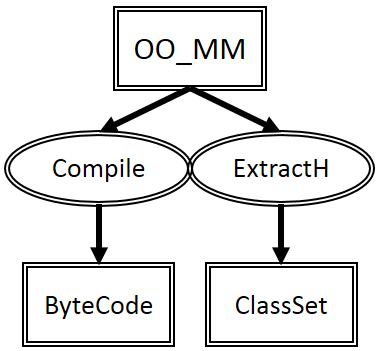
\includegraphics[width=0.1\textwidth]{OO_FTG}
  \end{center}
  \caption{Simple \textsc{Ftg}: compilation and hierarchy extraction.}
  \label{fig:OO_FTG}
\end{wrapfigure}
Figure \ref{fig:OO_FTG} pictures a simple \textsc{Ftg} using two template, 
automatic transformations (names) (represented with double-rounded, white 
items) called $\mathsf{Compile}, \mathsf{ExtractH}\in 
\mathsf{TTransName}$ that respectively compile and extract the class hierarchy 
of a template metamodel $\mathsf{OO\_MM}\in\mathsf{TMMName}$. 

\medskip
As its name indicates, a \textsc{Pm} describes a process, i.e., a set of 
activities that are combined together towards achieving a particular goal. 
Instead of reinventing a Domain-Specific Language for this well-studied domain, 
we simply specialise one standard and well-known language that covers our 
needs, namely \textsc{Uml}'s Activity Diagrams.


%%%%%%%%%%%%%%%%%%%%
% PROCESS MODEL
%%%%%%%%%%%%%%%%%%%%
\begin{Definition}[\label{def:PM}Process Model (\textsc{Pm})]
% %
A \emph{process model} $\mathsf{P}\in\PM$ is an instance of a \textsc{Uml}
Activity Diagram where
\begin{itemize}
   \item $\mathsf{ActionNode}$s are labelled by transformation instance names 
typed by their conforming transformation specifications, and may be 
\emph{hierarchical} and may contain input/output $\mathsf{Pin}$s; and 
   \item $\mathsf{ObjectNode}$s are labelled by language instance names typed 
by their conforming languages; and 
   \item $\mathsf{ControlNode}$s include 
$\mathsf{Decision}$/$\mathsf{Merge}$, $\mathsf{Fork}$/$\mathsf{Join}$ and 
$\mathsf{Init}$/$\mathsf{Final}$s nodes.   
\end{itemize}
%%
\end{Definition}
\begin{wrapfigure}[9]{r}{0.1\textwidth}
  \begin{center}
    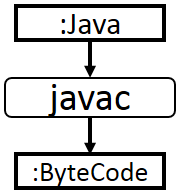
\includegraphics[width=0.1\textwidth]{OO_PM}
  \end{center}
  \caption{Simple compiling \textsc{PM}.}
  \label{fig:OO_PM}
\end{wrapfigure}
Figure \ref{fig:OO_PM} pictures a compilation process between one 
$\mathsf{ObjectNode}$ representing a Java program $\mathsf{:Java}$ producing a 
ByteCode instance $\mathsf{:ByteCode}$ through the  $\mathsf{ActionNode}$ 
$\mathsf{javac}$.

\medskip
The following definition simply puts things together: a workflow is composed of 
an \textsc{Ftg} together with a \emph{well-formed} \textsc{Pm}. 



%%%%%%%%%%%%%%%%%%%%
% WORKFLOW
%%%%%%%%%%%%%%%%%%%%
\begin{Definition}[\label{def:Workflow}Workflow]
   A \emph{workflow} $\mathsf{W}\in\mathbb{W}(TR, MM)$ is a pair $\mathsf{W} = 
(\mathsf{FTG}, \mathsf{P})$ where $\mathsf{FTG}\in\FTG(TR, MM)$ and 
$\mathsf{P}\in\PM$, such that $\mathsf{P}$ is well-formed (noted 
$\mathsf{P} \blacktriangleright \mathsf{FTG}$) wrt. $\mathsf{FTG}$, i.e. for 
each $\mathsf{ActionNode}$ inside $\mathsf{P}$ with name 
$tr$,
\begin{itemize}
   \item there exists a transformation (name) $\mathsf{t}\in 
\Dom{\mathsf{FTG}}$ in the domain of $\mathsf{FTG}$, that refers to a 
transformation $tr$ conforms to, up to a matching morphism (i.e. 
$tr \rhd trans(\mathsf{t})$, or $tr \rhd \mathsf{MM}$ such that $\mathsf{MM} 
\rightsquigarrow tt(\mathsf{tr})$).
  
   \item for each source or target $fl_i$ of $t$ at rank $i$ with (template) 
metamodel $\mathsf{MM_i}$, there exists a $\mathsf{Pin}$ at rank $i$ connected 
(as input or output) to an $\mathsf{ObjectNode}$ carrying a model 
$model(\mathsf{mname}) \in \mathbb{M}$ conform to a metamodel $\mathsf{MM'}$ 
(i.e. $\mathsf{M} \rhd \mathsf{MM'}$) such that either $\mathsf{MM}$ is the 
$i$-metamodel of $tr$ (i.e. $\mathsf{MM} = \mathsf{MM'}$), or it matches it 
(i.e. $\mathsf{MM} \rightsquigarrow \mathsf{MM}$).

% typed by a language 
% $\mathsf{L}\in\mathbb{L}$, such that 
% $\mathsf{LI} \;\rhd\; \mathsf{L}$, and $\mathsf{L}\rightsquigarrow F$, then one 
% of the following holds:
%    \begin{itemize}
%       \item $fl_i\in \mathsf{AbstractFormalismN}$ then $fl_i$ denotes an 
% abstract formalism that should refine (some 
% of) the formalisms implemented by $\mathsf{L}$, i.e. $form(fl_i) \sqsubseteq 
% \mathsf{F'_{k_1}}, \ldots form(fl_i) \sqsubseteq \mathsf{F'_{k_n}}$ such that 
% $\mathsf{F'_{k_1}}, \ldots \mathsf{F'_{k_n}} \subseteq F$;
%       
%       \item $fl_i\in \mathsf{LanguageN}$ then $fl_i$ denotes a language. The 
% language that should refine $\mathsf{L}$ i.e. $lang(fl_i) \sqsubseteq 
% \mathsf{L}$.
%    \end{itemize}
\end{itemize}
\end{Definition}
\noindent
When clear from context, or unnecessarily detailed, we simply note the set of 
workflows $\mathbb{W}$, without any indication of languages or 
transformations (sets).

As illustration, the \textsc{Pm} in Fig. \ref{fig:OO_PM} is well-formed wrt. 
the \textsc{Ftg} in Fig. \ref{fig:OO_FTG}: as established earlier, 
$\mathsf{:\!Java}$ refers to a Java model, whose metamodel matches 
$\mathsf{OO\_MM}$ and $\mathsf{javac}$ is an appropriate match for 
$\mathsf{Compile}$; furthermore, no transformation (execution) are exhibited for 
matching $\mathsf{ExtractH}$.

Our definition for x\textsc{Ftg}s relies solely on \emph{names}: we heavily 
rely on the repository (Modelverse) capabilities in order to first retrieve the 
appropriate items (metamodels, models and transformations) as well as checking 
that matching between them is appropriately achieved. This was abstracted away 
in Def. \ref{def:Naming}, but requires a proper formalisation in the future.

Similar to the original  
\cite{Mustafiz-etAl:2012,Lucio-Mustafiz-etAl:2013,TR:Lucio-Mustafiz-etAl:2012},
our definition does not impose a particular topology on the $\mathsf{PM}$ as 
long as transformations are well-formed. However, the original definition 
simply rely on a name-matching typing, similar to what is depicted in Fig. 
\ref{fig:OO_PM}, leverage \UML{}-like Object/Class instanciation. In contrast, 
we introduced a relaxed matching mechanism based on metamodel/transformation 
matching relying on the $\rightsquigarrow$ relationship.

%%%%%%%%%%%%%%%%%%%%%%%%%%%%%%%%%%%%%%%%%%%%%%%%%%%%%%%%%%%%%%%%%%%%%%%%%%%%
\subsection{Paradigm}
\label{sec:PS}

Properties characterising a paradigm (as briefly described in Table 
\ref{tab:Properties}) may span over all the previous elements: for example, 
expressing the inheritance formally would require to have at disposal the 
(template) metamodel of Fig. \ref{fig:InheritenceTemplate}, but also access to 
its semantic domain to check that the state of a superclass becomes available 
to all objects of any subclass. Similarly, properties over transformations may 
restrict or constraint its applicability (e.g., $\mathsf{ExtractH}$ would have 
to define preconditions for object-oriented metamodels allowing multiple 
inheritance, and have a postcondition on the datastructure of its output). 
Properties may also characterise the topology, the usage and the matching 
process in an \textsc{Ftg} or its corresponding \textsc{Pm} (by, for example, 
ensuring frequent loops for the Agile paradigm). 

We first collect all previous elements in a single mathematical structure 
called \emph{paradigmatic structure} on which properties may hold.

%%%%%%%%%%%%%%%%%%%%
% PARAD. STRUCTURE
%%%%%%%%%%%%%%%%%%%%

\begin{Definition}[Paradigmatic Structure]
   A \emph{paradigmatic structure} $\mathsf{PS}\in \PS$ is a pair $\mathsf{PS} 
= (MM, W)$ where $MM\in \wp(\mathcal{M})$ is a set of metamodels and 
$W \in \wp(\mathbb{W})$ is a set of workflows.
\end{Definition}

% Table \ref{tab:Properties} already described some interesting properties 
% related to three well-known paradigms. As easily noticeable, properties span 
% over all elements constituting a paradigmatic structure: the components of the 
% languages involved (and potentially, properties that require certain 
% combinations of languages); transformations; and also the processes. Some 
% paradigms may also have ''sanity-check`` properties that characterise the 
% paradigm itself. We will call these properties capturing the essence of a 
% paradigm \emph{paradigmatic properties}.

Following the mantra of modelling ''at the most appropriate 
level of abstraction``, it becomes impossible at the abstraction level of this 
presentation to formally (i.e., intensionally) define the nature of such a 
large class of properties. We therefore provide an extensional definition: we 
note $\mathcal{P}(S)$ the set of all possible properties expressible over a 
structure $S$. 

%%%%%%%%%%%%%%%%%%% 
% PARAD. PROPERTIES 
%%%%%%%%%%%%%%%%%%%

\begin{Definition}[\label{def:ParaProperties}Paradigmatic Properties]
   A \emph{paradigmatic property} is a tuple
$\pi = (\pi_{\mathsf{MM}},\pi_{\mathsf{W}},\pi_{\mathsf{PS}}) \in \Pi$ where
\begin{itemize}
   \item $\pi_{\mathsf{MM}} \in \mathcal{P}(\mathcal{M})$ is a set of 
properties 
over metamodels (and their semantics);
   \item $\pi_{\mathsf{W}} \in \mathcal{P}(\mathbb{W})$ is a set of properties 
over workflows (and their matching procedure);
   \item $\pi_{\mathsf{PS}}\in\mathcal{P}(\PS)$ is a set of 
properties spanning over all components of paradigmatic structures).
\end{itemize}
\end{Definition}
\noindent
Paradigmatic properties may be expressed through \emph{pattern languages}, 
e.g., 
for ensuring the presence of certain concepts, or through \emph{dedicated 
logics}, e.g., for ensuring semantic properties. 
% We detail later in the examples how some properties described in Table 
% \ref{tab:Properties} may be captured precisely.

We finally associate a \emph{name} to a set of properties for referring to a 
specific paradigm.
\begin{Definition}{\label{def:Paradigm}Paradigm}
Let $\mathsf{ParadigmName}$ be a set of (paradigm) names, that we associate to 
properties through a function $\iota \in [\mathsf{IntentN} \to \Pi]$.

For $\mathsf{paradigm}\in\mathsf{ParadigmName}$ such that 
$\iota(\mathsf{paradigm}) = (\pi_{\mathsf{MM}}(\mathsf{p}),                     
 \pi_{\mathsf{W}}(\mathsf{p}),                      
\pi_{\mathsf{PS}}(\mathsf{p}))$, 
we say that $\mathsf{PS} = (MM, W)\in\PS$ \emph{embodies} (alternatively, 
\emph{follows}, \emph{qualifies as}) $\mathsf{paradigm}$ iff
\begin{itemize}
   \item the properties $\pi_{\mathsf{MM}}(\mathsf{p})$ hold on $MM$;
   \item the properties $\pi_{\mathsf{W}}(\mathsf{p})$ hold on $W$; and
   \item the properties $ \pi_{\mathsf{PS}}(\mathsf{p}))$ hold on $\mathsf{PS}$.
\end{itemize}
\end{Definition}
Notice that it may be interesting to introduce namespaces for paradigm names, 
since it is likely that similar denominations would be used for slightly 
different sets of properties: for example, one may define object orientation in 
the context of single or multiple inheritance, the latter requiring to take 
care of conflicting properties (as it is with the renaming mechanism in Eiffel).

